\section{Introduction}\label{introduction}

\begin{frame}{Good Quote}

\begin{quote}
``You must stick to your conviction, but be ready to abandon your
assumptions.''

--- Dennis Waitley
\end{quote}

\end{frame}

\begin{frame}{GLMs}

Generalized Linear Models (GLMs):

\begin{enumerate}
\def\labelenumi{\arabic{enumi}.}
\tightlist
\item
  Are extensions of linear regression to areas where assumptions of
  normality and homoskedasticity do not hold
\item
  There are several versions of GLM's, each for different types and
  distributions of outcomes.
\end{enumerate}

We are going to go through several of the most common GLMs.

\end{frame}

\begin{frame}{Types}

We discuss:

\begin{enumerate}
\def\labelenumi{\arabic{enumi}.}
\tightlist
\item
  Logistic Regression
\item
  Poisson Regression
\item
  GLM with Gamma distribution
\item
  Negative binomial
\item
  Beta Regression
\end{enumerate}

\end{frame}

\section{Logistic Regression}\label{logistic-regression}

\begin{frame}[fragile]{Logistic Regression}

For binary outcomes (e.g., yes or no, correct or incorrect, sick or
healthy)

\begin{Shaded}
\begin{Highlighting}[]
\NormalTok{## First creating binary depression variable}
\NormalTok{df <-}\StringTok{ }\NormalTok{df }\OperatorTok
\StringTok{  }\KeywordTok{mutate}\NormalTok{(}\DataTypeTok{dep =}\NormalTok{ dpq010 }\OperatorTok{+}\StringTok{ }\NormalTok{dpq020 }\OperatorTok{+}\StringTok{ }\NormalTok{dpq030 }\OperatorTok{+}\StringTok{ }\NormalTok{dpq040 }\OperatorTok{+}\StringTok{ }\NormalTok{dpq050 }\OperatorTok{+}
\StringTok{               }\NormalTok{dpq060 }\OperatorTok{+}\StringTok{ }\NormalTok{dpq070 }\OperatorTok{+}\StringTok{ }\NormalTok{dpq080 }\OperatorTok{+}\StringTok{ }\NormalTok{dpq090) }\OperatorTok
\StringTok{  }\KeywordTok{mutate}\NormalTok{(}\DataTypeTok{dep2 =} \KeywordTok{ifelse}\NormalTok{(dep }\OperatorTok{>=}\StringTok{ }\DecValTok{10}\NormalTok{, }\DecValTok{1}\NormalTok{,}
                \KeywordTok{ifelse}\NormalTok{(dep }\OperatorTok{<}\StringTok{ }\DecValTok{10}\NormalTok{, }\DecValTok{0}\NormalTok{, }\OtherTok{NA}\NormalTok{)))}
\end{Highlighting}
\end{Shaded}

Note:

\begin{enumerate}
\def\labelenumi{\arabic{enumi}.}
\tightlist
\item
  IF depression \(\geq 10\) then dep2 is 1,
\item
  IF dpression \(< 10\), then dep2 is 0,
\item
  ELSE dep2 is NA.
\end{enumerate}

\end{frame}

\begin{frame}[fragile]{Running Logistic Regression}

Since the outcome is binary, we use a statistical transformation to make
things work well. This makes it so the outcome is in ``log-odds.'' A
simple exponentiation of the coefficients and we get very useful ``odds
ratios.''

Luckily, running a logistic regression is simple in \texttt{R}. We first
create the binary outcome variable called \texttt{dep}. We use a new
function called \texttt{mutate} to create a new variable (we could do
this a number of ways but this is probably the cleanest way).

\end{frame}

\begin{frame}[fragile]{Running Logistic Regression}

\begin{Shaded}
\begin{Highlighting}[]
\NormalTok{## Fix some placeholders}
\NormalTok{df <-}\StringTok{ }\NormalTok{df }\OperatorTok
\StringTok{  }\KeywordTok{mutate}\NormalTok{(}\DataTypeTok{asthma =} \KeywordTok{washer}\NormalTok{(mcq010, }\DecValTok{9}\NormalTok{),}
         \DataTypeTok{asthma =} \KeywordTok{washer}\NormalTok{(asthma, }\DecValTok{2}\NormalTok{, }\DataTypeTok{value =} \DecValTok{0}\NormalTok{)) }\OperatorTok
\StringTok{  }\KeywordTok{mutate}\NormalTok{(}\DataTypeTok{sed =} \KeywordTok{washer}\NormalTok{(pad680, }\DecValTok{9999}\NormalTok{, }\DecValTok{7777}\NormalTok{))}
\end{Highlighting}
\end{Shaded}

\end{frame}

\begin{frame}[fragile]{Running Logistic Regression}

Now let's run the logistic regression: \small

\begin{Shaded}
\begin{Highlighting}[]
\NormalTok{l_fit <-}\StringTok{ }\KeywordTok{glm}\NormalTok{(dep2 }\OperatorTok{~}\StringTok{ }\NormalTok{asthma }\OperatorTok{+}\StringTok{ }\NormalTok{sed }\OperatorTok{+}\StringTok{ }\NormalTok{race }\OperatorTok{+}\StringTok{ }\NormalTok{famsize,}
             \DataTypeTok{data =}\NormalTok{ df,}
             \DataTypeTok{family =} \StringTok{"binomial"}\NormalTok{)}
\KeywordTok{summary}\NormalTok{(l_fit)}
\end{Highlighting}
\end{Shaded}

\begin{verbatim}
## 
## Call:
## glm(formula = dep2 ~ asthma + sed + race + famsize, family = "binomial", 
##     data = df)
## 
## Deviance Residuals: 
##     Min       1Q   Median       3Q      Max  
## -0.7831  -0.4479  -0.4078  -0.3645   2.5471  
## 
## Coefficients:
##                     Estimate Std. Error z value Pr(>|z|)    
## (Intercept)       -2.6203555  0.2380770 -11.006  < 2e-16 ***
## asthma             0.5688452  0.1276326   4.457 8.32e-06 ***
## sed                0.0005638  0.0002610   2.160   0.0307 *  
## raceOtherHispanic  0.7162568  0.2328673   3.076   0.0021 ** 
## raceWhite          0.1287059  0.2116414   0.608   0.5431    
## raceBlack          0.0189205  0.2205461   0.086   0.9316    
## raceOther         -0.4901414  0.2570123  -1.907   0.0565 .  
## famsize           -0.0318309  0.0373218  -0.853   0.3937    
## ---
## Signif. codes:  0 '***' 0.001 '**' 0.01 '*' 0.05 '.' 0.1 ' ' 1
## 
## (Dispersion parameter for binomial family taken to be 1)
## 
##     Null deviance: 2706.3  on 4436  degrees of freedom
## Residual deviance: 2648.2  on 4429  degrees of freedom
##   (195 observations deleted due to missingness)
## AIC: 2664.2
## 
## Number of Fisher Scoring iterations: 5
\end{verbatim}

\normalsize

\end{frame}

\begin{frame}[fragile]{Output of Logistic Regression}

We used \texttt{glm()} (stands for generalized linear model)

The key to making it logistic, since you can use \texttt{glm()} for a
linear model using maximum likelihood instead of \texttt{lm()} with
least squares, is \texttt{family\ =\ "binomial"}

\end{frame}

\section{Poisson Regression}\label{poisson-regression}

\begin{frame}[fragile]{Poisson Regression}

Again, we will use the \texttt{glm()} function.

The difference here is we will be using an outcome that is a count
variable. For example, the sedentary variable (\texttt{sed}) that we
have in \texttt{df} is a count of the minutes of sedentary activity.

\end{frame}

\begin{frame}[fragile]{Running Poisson Regression}

\tiny

\begin{Shaded}
\begin{Highlighting}[]
\NormalTok{p_fit <-}\StringTok{ }\KeywordTok{glm}\NormalTok{(sed }\OperatorTok{~}\StringTok{ }\NormalTok{asthma }\OperatorTok{+}\StringTok{ }\NormalTok{race }\OperatorTok{+}\StringTok{ }\NormalTok{famsize,}
             \DataTypeTok{data =}\NormalTok{ df,}
             \DataTypeTok{family =} \StringTok{"poisson"}\NormalTok{)}
\KeywordTok{summary}\NormalTok{(p_fit)}
\end{Highlighting}
\end{Shaded}

\begin{verbatim}
## 
## Call:
## glm(formula = sed ~ asthma + race + famsize, family = "poisson", 
##     data = df)
## 
## Deviance Residuals: 
##     Min       1Q   Median       3Q      Max  
## -27.362   -8.430   -1.477    5.823   34.507  
## 
## Coefficients:
##                     Estimate Std. Error z value Pr(>|z|)    
## (Intercept)        5.6499871  0.0035550 1589.31   <2e-16 ***
## asthma             0.0614965  0.0021434   28.69   <2e-16 ***
## raceOtherHispanic  0.1393438  0.0040940   34.04   <2e-16 ***
## raceWhite          0.3484622  0.0033438  104.21   <2e-16 ***
## raceBlack          0.3400346  0.0034430   98.76   <2e-16 ***
## raceOther          0.3557953  0.0036273   98.09   <2e-16 ***
## famsize           -0.0188673  0.0005488  -34.38   <2e-16 ***
## ---
## Signif. codes:  0 '***' 0.001 '**' 0.01 '*' 0.05 '.' 0.1 ' ' 1
## 
## (Dispersion parameter for poisson family taken to be 1)
## 
##     Null deviance: 496351  on 4436  degrees of freedom
## Residual deviance: 475428  on 4430  degrees of freedom
##   (195 observations deleted due to missingness)
## AIC: 508999
## 
## Number of Fisher Scoring iterations: 5
\end{verbatim}

\normalsize

\end{frame}

\begin{frame}{Running Poisson Regression}

Sedentary may be over-dispersed:
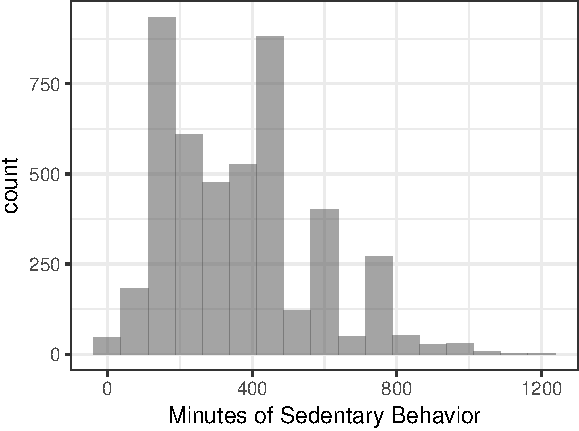
\includegraphics{05_GeneralizedLinearModels_files/figure-beamer/unnamed-chunk-6-1.pdf}
and so other methods related to poisson may be necessary. For this book,
we are not going to be delving into these in depth but we will introduce
some below.

\end{frame}

\begin{frame}[fragile]{Gamma}

\begin{itemize}
\tightlist
\item
  very similar to poisson but does not require integers and can handle
  more dispersion.
\item
  the outcome must have values \(> 0\).
\end{itemize}

\small

\begin{Shaded}
\begin{Highlighting}[]
\NormalTok{## Adjust sed}
\NormalTok{df}\OperatorTok{$}\NormalTok{sed_gamma <-}\StringTok{ }\NormalTok{df}\OperatorTok{$}\NormalTok{sed }\OperatorTok{+}\StringTok{ }\NormalTok{.}\DecValTok{01}
\NormalTok{g_fit <-}\StringTok{ }\KeywordTok{glm}\NormalTok{(sed_gamma }\OperatorTok{~}\StringTok{ }\NormalTok{asthma }\OperatorTok{+}\StringTok{ }\NormalTok{race }\OperatorTok{+}\StringTok{ }\NormalTok{famsize,}
             \DataTypeTok{data =}\NormalTok{ df,}
             \DataTypeTok{family =} \StringTok{"Gamma"}\NormalTok{)}
\KeywordTok{summary}\NormalTok{(g_fit)}
\end{Highlighting}
\end{Shaded}

\begin{verbatim}
## 
## Call:
## glm(formula = sed_gamma ~ asthma + race + famsize, family = "Gamma", 
##     data = df)
## 
## Deviance Residuals: 
##     Min       1Q   Median       3Q      Max  
## -4.3589  -0.4613  -0.0845   0.2926   1.6868  
## 
## Coefficients:
##                     Estimate Std. Error t value Pr(>|t|)    
## (Intercept)        3.567e-03  1.132e-04  31.515  < 2e-16 ***
## asthma            -1.604e-04  5.865e-05  -2.735  0.00626 ** 
## raceOtherHispanic -4.874e-04  1.309e-04  -3.723  0.00020 ***
## raceWhite         -1.090e-03  1.078e-04 -10.115  < 2e-16 ***
## raceBlack         -1.068e-03  1.102e-04  -9.697  < 2e-16 ***
## raceOther         -1.110e-03  1.145e-04  -9.695  < 2e-16 ***
## famsize            5.107e-05  1.552e-05   3.289  0.00101 ** 
## ---
## Signif. codes:  0 '***' 0.001 '**' 0.01 '*' 0.05 '.' 0.1 ' ' 1
## 
## (Dispersion parameter for Gamma family taken to be 0.2932604)
## 
##     Null deviance: 1664.8  on 4436  degrees of freedom
## Residual deviance: 1604.2  on 4430  degrees of freedom
##   (195 observations deleted due to missingness)
## AIC: 59154
## 
## Number of Fisher Scoring iterations: 5
\end{verbatim}

\normalsize

\end{frame}

\begin{frame}[fragile]{Two-Part or Hurdle Models}

We are going to use the \texttt{pscl} package to run a hurdle model.
These models are built for situations where there is a count variable
with many zeros (``zero-inflated''). The hurdle model makes slightly
different assumptions regarding the zeros than the pure negative
binomial that we present next. The hurdle consists of two models: one
for whether the person had a zero or more (binomial) and if more than
zero, how many (poisson).

To run a hurdle model, we are going to make a sedentary variable with
many more zeros to illustrate and then we will run a hurdle model.

\small

\begin{Shaded}
\begin{Highlighting}[]
\NormalTok{## Zero inflated sedentary (don't worry too much about the specifics)}
\NormalTok{df}\OperatorTok{$}\NormalTok{sed_zero <-}\StringTok{ }\KeywordTok{ifelse}\NormalTok{(}\KeywordTok{sample}\NormalTok{(}\DecValTok{1}\OperatorTok{:}\DecValTok{100}\NormalTok{, }
                             \DataTypeTok{size =} \KeywordTok{length}\NormalTok{(df}\OperatorTok{$}\NormalTok{sed), }
                             \DataTypeTok{replace=}\OtherTok{TRUE}\NormalTok{) }\OperatorTok\StringTok{ }\KeywordTok{c}\NormalTok{(}\DecValTok{5}\NormalTok{,}\DecValTok{10}\NormalTok{,}\DecValTok{11}\NormalTok{,}\DecValTok{20}\OperatorTok{:}\DecValTok{25}\NormalTok{), }\DecValTok{0}\NormalTok{, }
\NormalTok{                      df}\OperatorTok{$}\NormalTok{sed)}
\NormalTok{## Hurdle model}
\KeywordTok{library}\NormalTok{(pscl)}
\NormalTok{h_fit =}\StringTok{ }\KeywordTok{hurdle}\NormalTok{(sed_zero }\OperatorTok{~}\StringTok{ }\NormalTok{asthma }\OperatorTok{+}\StringTok{ }\NormalTok{race }\OperatorTok{+}\StringTok{ }\NormalTok{famsize,}
               \DataTypeTok{data =}\NormalTok{ df)}
\KeywordTok{summary}\NormalTok{(h_fit)}
\end{Highlighting}
\end{Shaded}

\begin{verbatim}
## 
## Call:
## hurdle(formula = sed_zero ~ asthma + race + famsize, data = df)
## 
## Pearson residuals:
##     Min      1Q  Median      3Q     Max 
## -3.9753 -1.5078 -0.2439  1.2588 10.7813 
## 
## Count model coefficients (truncated poisson with log link):
##                     Estimate Std. Error z value Pr(>|z|)    
## (Intercept)        5.6557869  0.0036967 1529.94   <2e-16 ***
## asthma             0.0550741  0.0022613   24.36   <2e-16 ***
## raceOtherHispanic  0.1164385  0.0042923   27.13   <2e-16 ***
## raceWhite          0.3405040  0.0034764   97.95   <2e-16 ***
## raceBlack          0.3437651  0.0035857   95.87   <2e-16 ***
## raceOther          0.3530576  0.0037635   93.81   <2e-16 ***
## famsize           -0.0203015  0.0005758  -35.26   <2e-16 ***
## Zero hurdle model coefficients (binomial with logit link):
##                   Estimate Std. Error z value Pr(>|z|)    
## (Intercept)        2.74919    0.22895  12.008   <2e-16 ***
## asthma            -0.07983    0.14420  -0.554   0.5798    
## raceOtherHispanic -0.29148    0.25258  -1.154   0.2485    
## raceWhite         -0.22787    0.21350  -1.067   0.2858    
## raceBlack         -0.44651    0.21650  -2.062   0.0392 *  
## raceOther          0.11825    0.24634   0.480   0.6312    
## famsize           -0.06432    0.03614  -1.780   0.0751 .  
## ---
## Signif. codes:  0 '***' 0.001 '**' 0.01 '*' 0.05 '.' 0.1 ' ' 1 
## 
## Number of iterations in BFGS optimization: 12 
## Log-likelihood: -2.327e+05 on 14 Df
\end{verbatim}

\normalsize

Notice that the output has two parts: ``Count model coefficients
(truncated poisson with log link):'' and ``Zero hurdle model
coefficients (binomial with logit link):''. Together they tell us about
the relationship between the predictors and a count variable with many
zeros.

\end{frame}

\begin{frame}[fragile]{Negative Binomial}

Similar to that above, negative binomial is for zero-inflated count
variables. It makes slightly different assumptions than the hurdle and
doesn't use a two-part approach. In order to run a negative binomial
model we'll use the \texttt{MASS} package and the \texttt{glm.nb()}
function.

\small

\begin{Shaded}
\begin{Highlighting}[]
\KeywordTok{library}\NormalTok{(MASS)}
\NormalTok{fit_nb <-}\StringTok{ }\KeywordTok{glm.nb}\NormalTok{(sed_zero }\OperatorTok{~}\StringTok{ }\NormalTok{asthma }\OperatorTok{+}\StringTok{ }\NormalTok{race }\OperatorTok{+}\StringTok{ }\NormalTok{famsize,}
                 \DataTypeTok{data =}\NormalTok{ df)}
\KeywordTok{summary}\NormalTok{(fit_nb)}
\end{Highlighting}
\end{Shaded}

\normalsize

Note that this model is not really appropriate because our data is
somewhat contrived.

\end{frame}

\section{Beta Regression}\label{beta-regression}

\begin{frame}{Beta Regression}

For outcomes that are bound between a lower and upper bound, Beta
Regression is a great method. For example, if we are looking at test
scores that are bound between 0 and 100. It is a very flexible method
and allows for some extra analysis regarding the variation.

\end{frame}

\begin{frame}[fragile]{Running Beta Regression}

For this, we are going to use the \texttt{betareg} package. But first,
we are going to reach a little and create a ficticiously bound variable
in the data set.

\begin{Shaded}
\begin{Highlighting}[]
\NormalTok{## Variable bound between 0 and 1}
\NormalTok{df}\OperatorTok{$}\NormalTok{beta_var <-}\StringTok{ }\KeywordTok{sample}\NormalTok{(}\KeywordTok{seq}\NormalTok{(.}\DecValTok{05}\NormalTok{, .}\DecValTok{99}\NormalTok{, }\DataTypeTok{by =}\NormalTok{ .}\DecValTok{01}\NormalTok{), }
                      \DataTypeTok{size =} \KeywordTok{length}\NormalTok{(df}\OperatorTok{$}\NormalTok{asthma),}
                      \DataTypeTok{replace =} \OtherTok{TRUE}\NormalTok{)}
\KeywordTok{library}\NormalTok{(betareg)}
\NormalTok{fit_beta <-}\StringTok{ }\KeywordTok{betareg}\NormalTok{(beta_var }\OperatorTok{~}\StringTok{ }\NormalTok{asthma }\OperatorTok{+}\StringTok{ }\NormalTok{race }\OperatorTok{+}\StringTok{ }\NormalTok{famsize,}
                    \DataTypeTok{data =}\NormalTok{ df)}
\KeywordTok{summary}\NormalTok{(fit_beta)}
\end{Highlighting}
\end{Shaded}

\end{frame}

\begin{frame}[fragile]{Running Beta Regression}

\begin{verbatim}
## 
## Call:
## betareg(formula = beta_var ~ asthma + race + famsize, data = df)
## 
## Standardized weighted residuals 2:
##     Min      1Q  Median      3Q     Max 
## -2.0937 -0.7133 -0.0425  0.6083  2.9121 
## 
## Coefficients (mean model with logit link):
##                    Estimate Std. Error z value Pr(>|z|)   
## (Intercept)        0.183438   0.063182   2.903  0.00369 **
## asthma             0.079145   0.043669   1.812  0.06993 . 
## raceOtherHispanic -0.028195   0.071914  -0.392  0.69501   
## raceWhite         -0.052655   0.058669  -0.897  0.36946   
## raceBlack         -0.013716   0.060909  -0.225  0.82184   
## raceOther          0.005879   0.065285   0.090  0.92825   
## famsize           -0.017376   0.010808  -1.608  0.10789   
## 
## Phi coefficients (precision model with identity link):
##       Estimate Std. Error z value Pr(>|z|)    
## (phi)  2.48105    0.04521   54.88   <2e-16 ***
## ---
## Signif. codes:  0 '***' 0.001 '**' 0.01 '*' 0.05 '.' 0.1 ' ' 1 
## 
## Type of estimator: ML (maximum likelihood)
## Log-likelihood:    92 on 8 Df
## Pseudo R-squared: 0.001691
## Number of iterations: 17 (BFGS) + 1 (Fisher scoring)
\end{verbatim}

The output provides coefficients and the ``Phi'' coefficients. Both are
important parts of using beta regression but we are not going to discuss
it here.

\end{frame}

\section{Conclusions}\label{conclusions}

\begin{frame}{Conclusions}

There are many resources available to learn more about beta regression
and each of these GLM's. As for now, we are going to move on to more
complex modeling where there are clustering or repeated measures in the
data.

\end{frame}

\begin{frame}[fragile]{Conclusions}

One of the great things about \texttt{R} is that most modeling is very
similar to the basic \texttt{lm()} function. In all of these GLM's the
arguments are nearly all the same: a formula, the data, and family of
model. As you'll see for Multilevel and Other Models chapters, this does
not change much. Having a good start with basic models and GLM's gets
you ready for nearly every other modeling type in \texttt{R}.

\end{frame}
